\documentclass[10pt,sigconf,letterpaper,nonacm]{acmart}
%\documentclass[10pt,sigconf,anonymous]{sig-alternate-10pt}
\settopmatter{printacmref=false}
\renewcommand\footnotetextcopyrightpermission[1]{} % remove footnote with conference information
\def\baselinestretch{0.98}
\setcopyright{none}
\pagestyle{plain} % remove running headers


\usepackage{subfigure,multirow}
\usepackage{graphicx}
\usepackage{url}
\usepackage{color}
\newcommand{\red}[1]{\textcolor{red}{#1}}
\newcommand{\blue}[1]{\textcolor{blue}{#1}}
\usepackage{array}
\usepackage{amsmath}
\usepackage{autobreak}
\usepackage{indentfirst} 

\newcommand{\tabincell}[2]{\begin{tabular}{@{}#1@{}}#2\end{tabular}}




\begin{document}
\bibliographystyle{plain}
\thispagestyle{empty}

\title{Presentation 1 report}
\author{Yihao Liu, Xiangyu Yin, Kai Huang}
\date{}
\maketitle

\section{Introduction}
Cardiac magnetic resonance imaging (MRI) is a unique non-ionizing radiation technique which provides clear view of heart’s anatomy. The anatomical information of MRI is useful in diagnosing cardiac disease. Whole heart segmentation (WHS) aims to extract the substructures of the heart, commonly including the four chamber blood cavities, the left ventricular myocardium, and sometimes the great vessels as well if they are of interest\cite{zheng2008four}. In order to automatically and accurately extract anatomical information, researchers nowadays are exploring novel algorithms in automatic WHS. 

However, Obtaining fully automatic WHS is arduous due to the low image quality and indistinct boundaries between substructures of the heart in cardiac MRI images. In order to solve this problem, Zhuang et. al\cite{zhuang2016multi} applies multi-modality atlas for whole heart segmentation. They utilize the cardiac CT images to help with the WHS of cardiac MRI images. Since CT is based on a different imaging principle than MRI, CT cardiac image is a good supplementary where the boundary in MRI image is blurry.  

\section{Implementation of multi-modality}
 Figure \ref{yihao_overview} shows the overview of multi-modality model in Zhuang's work\cite{zhuang2016multi}. The segmentation process is based on weighted label fusion(LWF). The key idea is to find the similarity between the training set and test images, and assign labels from maximum likelihood. The training images include MRI and CT images and are manually labeled with different cardiac regions. Since these images are from different individuals or taken at different perspective, each image should be aligned to a standard cardiac model by affine deformation. The label fusion result from each training image is weighted by the similarity to the target image. In order to have a clearer boundary, the test images are converted into entropy atlases using different patch sizes. These atlases are used as the input of a Gaussian regression model to output the mask of the boundary of heart. Finally, by combining the label fusion result and the mask, the target image is segmented by the LWF model.
 
 The entropy atlas are computed as follows\cite{wachinger2012entropy}. For each pixel in a cardiac image, a local patch centered on the pixel is selected. For each of these patches, one can compute its intensity entropy and store this entropy value in the location of the pixel to create a new image. Large patch size suppresses the fin structure but captures global structural information within a certain vision window, while small patch size provides more local details of the structure. The aim of utilizing different patch scales is to get the advantages of both scales.
 
 
 
 \section{Discussion}
 The model in Zhang et.al's work\cite{zhuang2016multi} is simple compared with complex data driven deep neural network. From our understanding, the key factor that affects the performance of WHS is whether we can obtain a clear boundary in MRI image. Thus, a GAN model is a more reasonable direction in multi-modality, whose aim is to convert the low quality cardiac images into high quality level. 

\begin{figure}
	\centering
	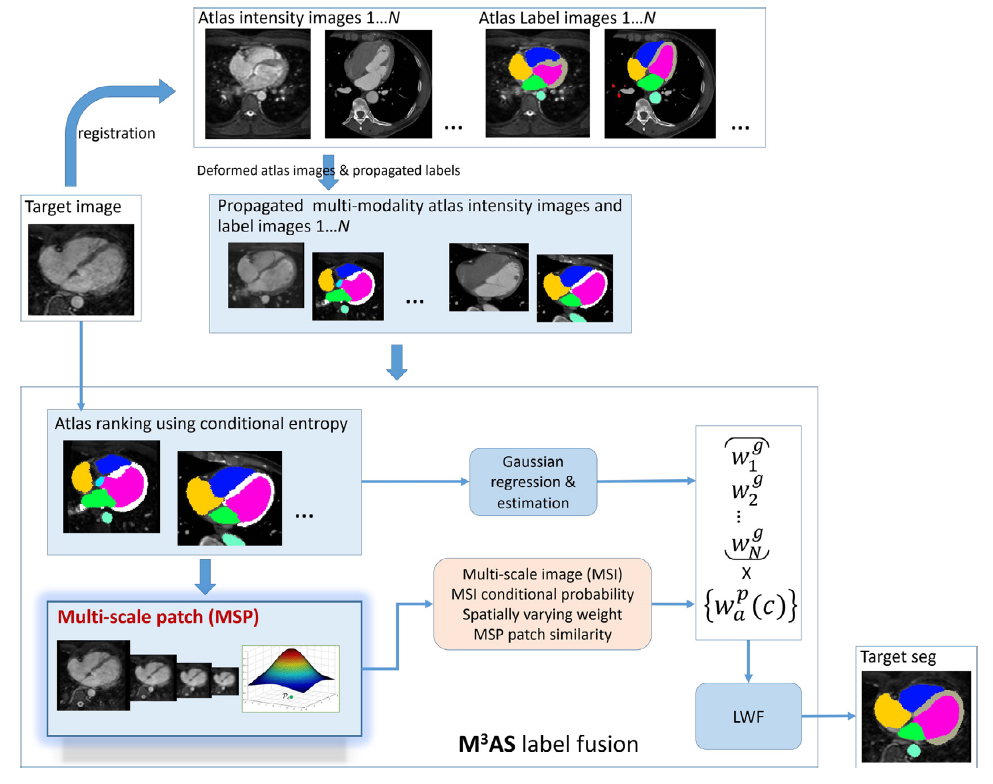
\includegraphics[width=0.4\textwidth]{images/yihao_overview.png}
	\caption{Overview of multi-modality model}
	\label{yihao_overview}
\end{figure} 




\setcounter{page}{1}

\bibliography{bibfile}
\end{document}


